\documentclass{report}

\begin{document}
	\section{Basic Terminology}
		\begin{defn}[Basic Terminology on Cryptosystems]
			\begin{itemize}
				\item[]
				\item \textbf{Plaintext}: The text before encryption
				\item \textbf{Ciphertext}: The text after encryption
				\item \textbf{Cryptosystems}: Encryption and decryption algorithms, see definition below for more
				\subitem \textbf{Encryption}: Using some sort of algorithm to change the content of a message so that it is unrecognizable.
				\subitem \textbf{Decryption}: Processing the encrypted message to change it back to the message.
				\item \textbf{Key}: A value required to encrypt or decrypt.
				\subitem \textbf{Encryption Key}: The key for encryption.
				\subitem \textbf{Decryption Key}: The key for decryption.
				\item \textbf{Cryptanalysis}: Decrypting the ciphertext without any prior knowledge(i.e. key).
			\end{itemize}
		\end{defn}
		
		\begin{defn}[Cryptosystem]
			A cryptosystem is defined as a set of three algorithms, $(G,E,D)$;
			\begin{itemize}
				\item[$G$]
				\subitem The key generation algorithm, sometimes abbreviated as \emph{KeyGen}, chooses the encryption key $k_1$ and the decryption key $k_2$ from the set of possible keys. The set of possible keys is called the \emph{key space}. Usually each key from the key space is chosen at uniformly random probability.
				\item[$E$]
				\subitem The Encryption Algorithm, sometimes abbreviated as \emph{Enc}, uses the encryption key $k_1$, takes the plaintext $m$ as an input, and produces the ciphertext $c$. This is usually denoted as follows:
				\begin{displaymath}
					E_{k_1}(m)=c
				\end{displaymath}
				\item[$D$]
				\subitem The Decryption Algorithm, sometimes abbreviated as \emph{Dec}, uses the decryption key $k_2$, takes the ciphertext $c$ as an input, and gains the plaintext $m$. This is usually denoted as follows:
				\begin{displaymath}
					D_{k_2}(c)=m
				\end{displaymath}
			\end{itemize}
			For a cryptosystem to be valid, by encrypting the plaintext $m$ and decrypting the ciphertext, we must be able to get $m$, that is;
			\begin{displaymath}
				D_{k_2}(E_{k_1}(m))=m
			\end{displaymath}
		\end{defn}
		
		A cryptosystem is classified into two categories; if the encryption key is the same as the decryption key, it is called a \emph{Symmetric Key Algorithm}; if not, it is called an \emph{Asymmetric Key Algorithm} or a \emph{Public Key Algorithm}. A symmetric key algorithm is again classified into two categories; \emph{Block Cipher} and \emph{Stream Cipher}.
		
		\begin{defn}[Kerckhoffs' Principle]
			Kerckhoffs' Principle states that a cryptosystem must be secure even if everything about the cryptosystem except for the key is exposed.
		\end{defn}
		Kerckhoffs' Principle says that the cryptosystem's security must depend only on the secrecy of the key. Its core comes from the idea that ``The enemy knows the system``. In some, ``Security through obscurity``(i.e. hiding the cryptosystem itself) holds but Kerckhoffs' Principle has its value for the following reasons:
		\begin{enumerate}
			\item Storing a smaller sized key is easier than hiding the entire cryptosystem. Also the cryptosystem is not safe from reverse engineering, but keys are, as they are usually a random number.
			\item If the key is exposed, it is easier to change only the key, not the entire cryptosystem.
			\item A cryptosystem is often used for many users, and everybody using the same cryptosystem allows for more efficient usage of space.
			\item If the cryptosystem itself is kept a secret, if a problem arises(i.e. reverse engineering) to expose the cryptosystem, then the entire thing must be redesigned. This takes a lot of knowledge and time.
			\item A cryptosystem is made weak by a small mistake; these mistakes are not found before the cryptosystems are analyzed fully, which is most easily done by making the system public. If they are indeed made public, the cryptosystem can be checked for security, allowing for a more secure system.
		\end{enumerate}
		
	\section{Encryption of Arbitrary Length Message}
		\subsection{Padding}
		When using a block cipher, we need the length of the message to be an exact multiple of the length of the block used in the block cipher. If not, we use \emph{padding} to make the message longer to make it an exact multiple. There are many ways to do so, but:
		\begin{itemize}
			\item \emph{Zero Padding}, otherwise known as \emph{Null Padding}
			\subitem Pad the message with zero($00$) bytes to make the length be an exact multiple of the cipher block length. This may cause a problem if the last bytes of the message are $00$.
			
			\item \emph{Bit Padding}
			\subitem Pad the message with $10|00^n$, so that we can know the start of padding. We must pad the message even if its length is a multiple of the cipher block length.
			
			\item \emph{Byte Padding}
			\subitem Same as zero padding, except the last byte is equal to the length of padding, that is; if we require four more bytes, the padding is $00|00|00|04$. We must pad the message even if its length is a multiple of the cipher block length.
			
			\item \emph{PKCS\#7 Padding}
			\subitem Similar to byte padding, except every byte of the padding is equal to the length of padding, that is; if we require four more bytes, the padding is $04|04|04|04$.
		\end{itemize}
	
		\subsection{Modes of Operation}
			Sometimes we are required to encrypt a longer message than the length of the block. The plaintext are first padded using one of the techniques above, and the padded plaintext $P$ is separated into blocks of padding length, $P_1,P_2,\cdots,P_N$. They are then encrypted using the key $K$, sometimes with the help of the initialization vector $IV$, and produces the ciphertexts $C_1,C_2,\cdots,C_N$. There are five major ways to do this; ECB, CBC, CFB, OFB, and CTR.
			
			\subsubsection{Electronic Code Book(ECB)}
				ECB mode is the simplest mode of them all. They simply take each blocks and encrypt them separately. In equation:
				\begin{itemize}
					\item \textbf{Encryption} $C_i=E_K(P_i)$
					\item \textbf{Decryption} $P_i=D_K(C_i)$
				\end{itemize}
				\begin{figure}[h!]
					\centering
					\subfloat{{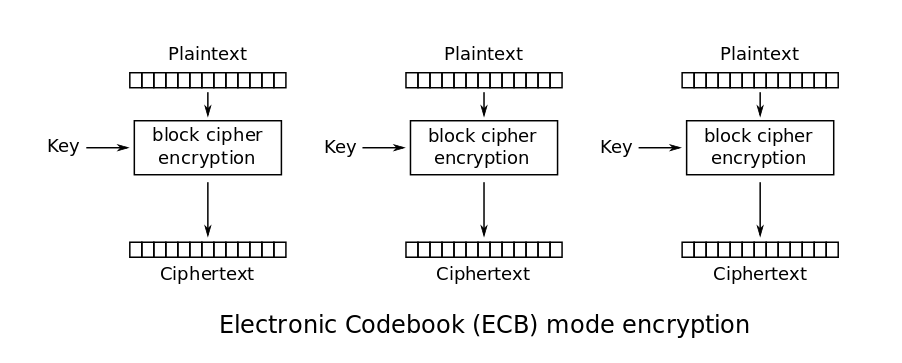
\includegraphics[width=0.47\linewidth]{./chapters/applications/mode-of-operation/ECB-ENC.png}}} \label{fig-ECB-ENC}
					\qquad
					\subfloat{{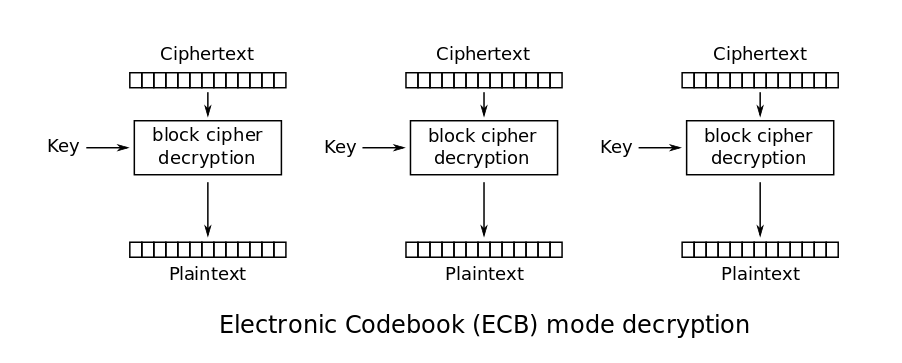
\includegraphics[width=0.47\linewidth]{./chapters/applications/mode-of-operation/ECB-DEC.png}}} \label{fig-ECB-DEC}
					\caption{ECB Mode}
					\label{fig-ECB}
				\end{figure}
				Since same plaintext blocks are encrypted into same ciphertext block, the blocks can be copied, or replayed, to change the message easily. This is called the \emph{Block Replay Attack}.

			\subsubsection{Cipher Block Chaining(CBC)}
				CBC takes the previous ciphertext block and XOR($\bigoplus$) it with the plaintext before encryption. The first block has no previous ciphertext block, hence it is XOR-ed with the $IV$. In equation:
				\begin{itemize}
					\item \textbf{Encryption} $C_0=IV$, $C_i=E_K(P_i \bigoplus C_{i-1}), i=1,2,3,\cdots,N$
					\item \textbf{Decryption} $C_0=IV$, $C_i=D_K(C_i) \bigoplus C_{i-1}, i=1,2,3,\cdots,N$
				\end{itemize}
				\begin{figure}[h!]
					\centering
					\subfloat{{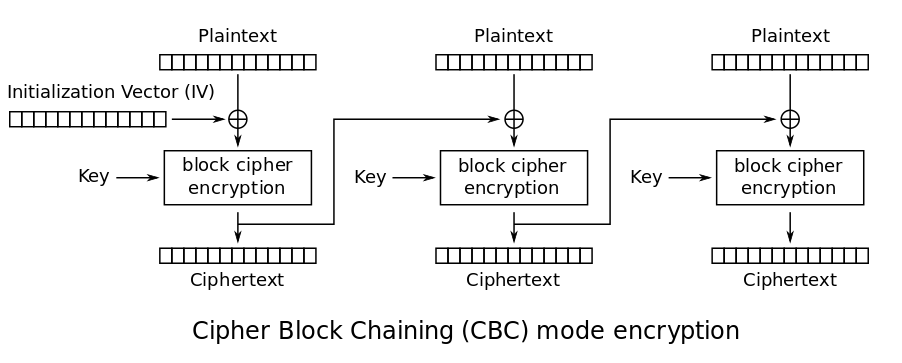
\includegraphics[width=0.47\linewidth]{./chapters/applications/mode-of-operation/CBC-ENC.png}}} \label{fig-CBC-ENC}
					\qquad
					\subfloat{{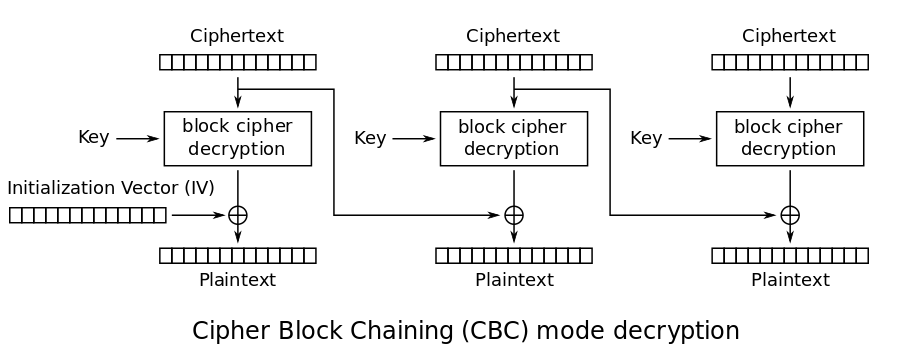
\includegraphics[width=0.47\linewidth]{./chapters/applications/mode-of-operation/CBC-DEC.png}}} \label{fig-CBC-DEC}
					\caption{CBC Mode}
					\label{fig-CBC}
				\end{figure}
			
			\subsubsection{Cipher Feedback(CFB)}
				CFB can be used to encrypt a block even smaller than the size of the encryption block, and can be used to make a stream cipher out of block cipher. In the diagram given below, original block sizes are used. In equation:
				\begin{itemize}
					\item \textbf{Encryption} $C_0=IV$, $C_i=E_K(P_i \bigoplus C_{i-1}), i=1,2,3,\cdots,N$
					\item \textbf{Decryption} $C_0=IV$, $C_i=D_K(C_i) \bigoplus C_{i-1}, i=1,2,3,\cdots,N$
				\end{itemize}
				\begin{figure}[h!]
					\centering
					\subfloat{{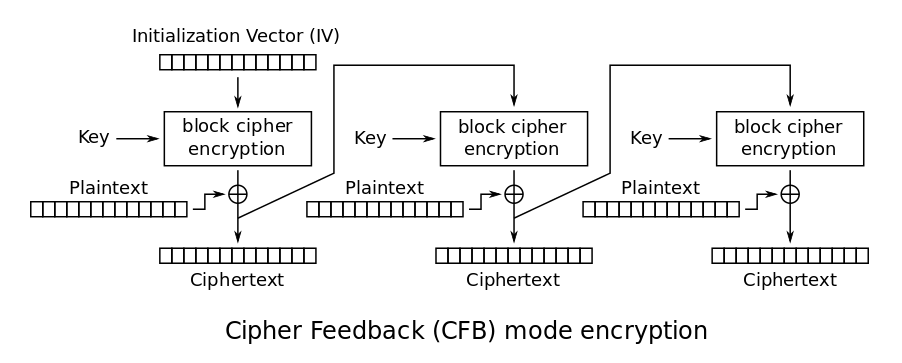
\includegraphics[width=0.47\linewidth]{./chapters/applications/mode-of-operation/CFB-ENC.png}}} \label{fig-CFB-ENC}
					\qquad
					\subfloat{{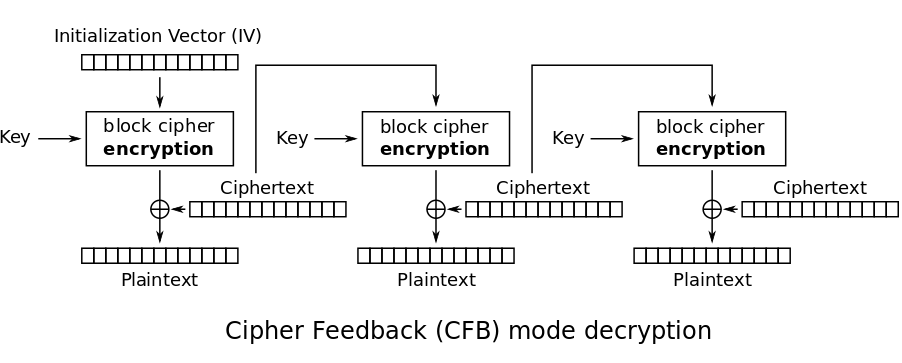
\includegraphics[width=0.47\linewidth]{./chapters/applications/mode-of-operation/CFB-DEC.png}}} \label{fig-CFB-DEC}
					\caption{CFB Mode}
					\label{fig-CFB}
				\end{figure}
				By altering the equation to the following we have the ``stream cipherized`` version, where $<<$ is the shift operation, $head(a,x)$ is the first $x$ bits of $a$, and $n$ is the size of the $IV$:
				\begin{itemize}
					\item \textbf{Shift Register} $S_0=IV$, $S_i=((S_i<<x)+C_i) \mod 2^n$
					\item \textbf{Encryption} $C_i=head(E_K(S_{i-1}),x) \bigoplus P_i$
					\item \textbf{Decryption} $P_i=head(E_K(S_{i-1}),x) \bigoplus C_i$
				\end{itemize}

			\subsubsection{Output Feedback(OFB)}
				OFB can be used to encrypt a block even smaller than the size of the encryption block, and can be used to make a stream cipher out of block cipher.
				\begin{itemize}
					\item \textbf{Input and Output} $I_0=IV$, $I_j=E_K(I_{j-1}), j=1,2,3,\cdots,N$
					\item \textbf{Encryption} $C_j=P_j \bigoplus I_j, i=1,2,3,\cdots,N$
					\item \textbf{Decryption} $P_j=C_j \bigoplus I_j, i=1,2,3,\cdots,N$
				\end{itemize}
				\begin{figure}[h!]
					\centering
					\subfloat{{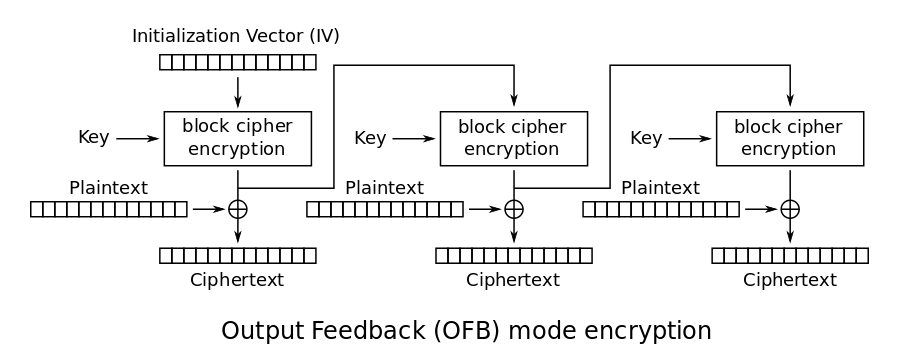
\includegraphics[width=0.47\linewidth]{./chapters/applications/mode-of-operation/OFB-ENC.png}}} \label{fig-OFB-ENC}
					\qquad
					\subfloat{{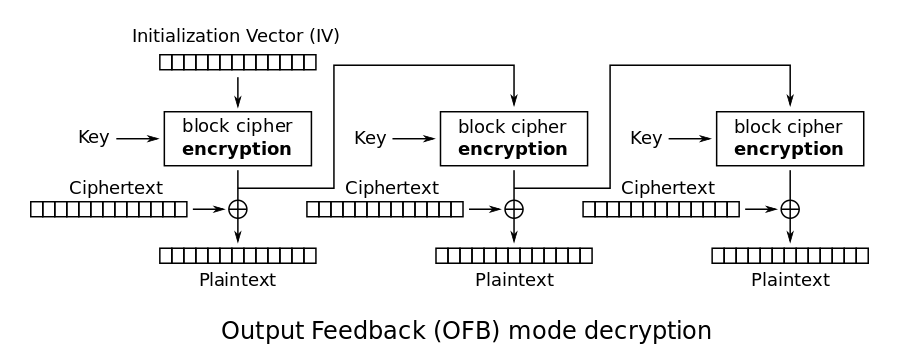
\includegraphics[width=0.47\linewidth]{./chapters/applications/mode-of-operation/OFB-DEC.png}}} \label{fig-OFB-DEC}
					\caption{OFB Mode}
					\label{fig-OFB}
				\end{figure}
				We can similarly alter the equation as OFB so that it can be used as a stream cipher.
			
			\subsubsection{Counter(CTR)}
				CTR can be used to encrypt a block even smaller than the size of the encryption block, and can be used to make a stream cipher out of block cipher. It encrypts the counter value instead of the plaintext, and XORs the value to gain the ciphertext.
				\begin{itemize}
					\item \textbf{Encryption} $C_i=P_i \bigoplus E_K(Counter), i=1,2,3,\cdots,N$
					\item \textbf{Decryption} $P_i=C_i \bigoplus E_K(Counter), i=1,2,3,\cdots,N$
				\end{itemize}
				\begin{figure}[h!]
					\centering
					\subfloat{{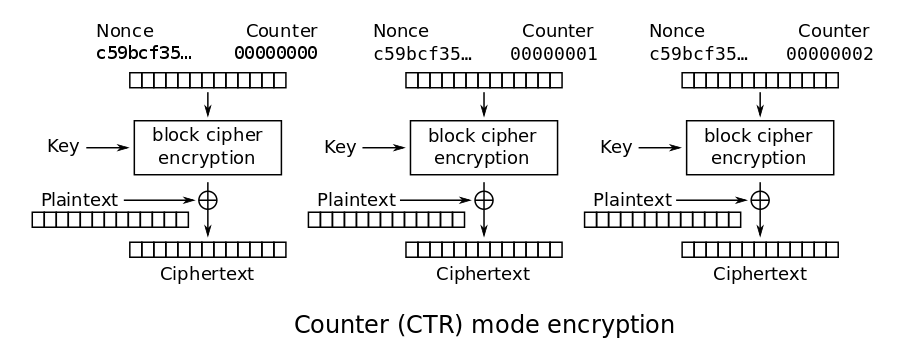
\includegraphics[width=0.47\linewidth]{./chapters/applications/mode-of-operation/CTR-ENC.png}}} \label{fig-CTR-ENC}
					\qquad
					\subfloat{{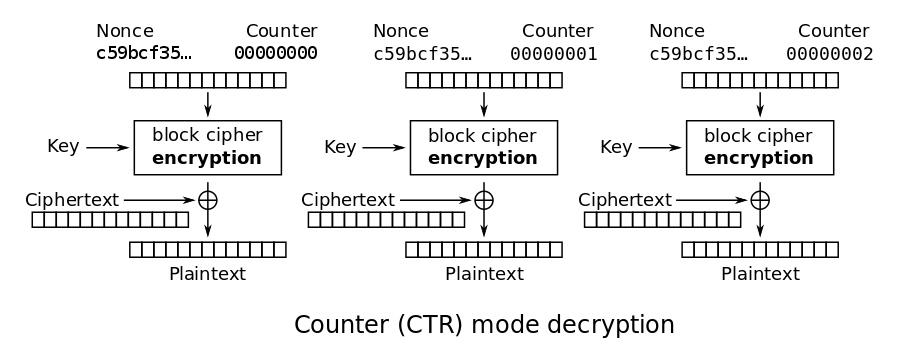
\includegraphics[width=0.47\linewidth]{./chapters/applications/mode-of-operation/CTR-DEC.png}}} \label{fig-CTR-DEC}
					\caption{CTR Mode}
					\label{fig-CTR}
				\end{figure}
				We can similarly alter the equation as OFB so that it can be used as a stream cipher.
			
				\subsubsection{Characteristics}
				Table \ref{table-mode-of-operation} shows the characteristics for each modes of operation.
				\begin{itemize}
					\item Block Pattern: Whether if the overall pattern is kept after encryption
					\item Preprocessing: Whether if preprocessing is possible on encryption and decryption
					\item Parallel Processing: Whether if parallel processing is possible on encryption or decryption
					\item Error Propagation: If there is an error in the encryption/decryption process, whether if the error spreads through other blocks
					\item Encryption Unit: The minimum requirement byte for encryption
				\end{itemize}
				\begin{table}[]
					\begin{tabular}{ccccccc}
						\multicolumn{2}{c}{}                              & ECB & CBC         & CFB         & OFB & CTR \\
						\multicolumn{2}{c}{Block Pattern}                 & O   & X           & X           & X   & X   \\
						\multicolumn{2}{c}{Preprocessing}                 & X   & X           & X           & O   & O   \\
						\multirow{2}{*}{Parallel Processing} & Encryption & O   & X           & X           & O   & O   \\
						& Decryption & O   & O           & O           & O   & O   \\
						\multicolumn{2}{c}{Error Propagation}             & X   & $(P_i,P_{i+1})$ & $\lceil \frac{n}{r} \rceil$ blocks & X   & X   \\
						\multicolumn{2}{c}{Encryption Unit}               & $n$   & $n$           & $r (\leq n)$           & $r (\leq n)$   & $r (\leq n)$  
					\end{tabular}
					\caption{Characteristics for Each Modes of Operation}
					\label{table-mode-of-operation}
				\end{table}
			
	\section{Types of Attack}
		\subsection{Attacking Classical Cryptosystems} 
			Classical Cryptosystems are typically a substitution cipher and/or a transposition cipher. Since most, if not all, the classical cryptosystems are broken, the two valid ways to attack any classical cryptosystems is given here.
			\begin{itemize}
				\item Brute Force Attack
				\subitem When the attacker gains the ciphertext $c$, the attacker uses every key possibility to try to gain $m$. This is otherwise known as the Exhaustive Key Search Attack. Theoretically this can be done to any symmetric-key cipher; but this is inapplicable to most modern cryptosystems as they have an extremely large key space.
				
				\item Frequency Analysis
				\subitem The plaintext having some pattern, such as the alphabet `e` appearing with the most frequency, will help the attacker gain knowledge on the plaintext just by seeing the ciphertext.
			\end{itemize}
		
	\section{Cryptographic Hash Functions}
		A general hash function has the following properties:
		\begin{itemize}
			\item They take an arbitrary size of data as input, and;
			\item They produce a constant and fixed length data as output.
		\end{itemize}
		A \emph{cryptographic hash function}, in addition to the properties above, must have the following properties:
		\begin{itemize}
			\item Preimage Resistance
			\subitem If the hash value $y$ is given, it must be hard to find an $x$ such that $h(x)=y$, that is, the hash function must have one-wayness.
			\item Second Preimage Resistance
			\subitem If the message $x$ is given, it must be hard to find an $x' \ne x$ such that $h(x)=h(x')$.
			\item Collision Resistance
			\subitem It must be hard to find $x \ne x'$ such that $h(x)=h(x')$. The pair $(x,x')$ is called the collision pair.
		\end{itemize}
		
	\section{Attacking the Cyrptosystems}
		Attacks on cryptosystems are classified into \emph{passive} and \emph{active} attack.
		Passive attacks simply eavesdrops the transmission, and gains what the attacker wants without modification of the message. This type of attacking includes \emph{eavesdropping}, of which the attacker intercepts the message in the middle to check the plaintext. This type of attacker is often referred to as "Eve"(as in eavesdropping) in theories.
		Active attackers will modify the message, which includes Modification, Deletion, Impersonation, and Replay. This type of attacker can also be referred to as "Eve", but sometimes is referred to as "Mallory", for malicious user.
		\begin{itemize}
			\item Modification: Changes the order of the message or changes a part of it to alter the meaning.
			\item Deletion: Intercepts the message and does not send it, interrupting the communication.
			\item Impersonation: Fakes their own identity to be identified as a correct user.
			\item Replay: Send a message again after eavesdropping, expecting some kind of result.
		\end{itemize}
		The four methods above are just the general ways to attack. We need to attack the system itself to know how to attack it. There are four methods of attack on system:
		\begin{itemize}
			\item \textbf{Ciphertext Only Attack}
			\subitem The attacker knows only the ciphertext.
			\item \textbf{Known Plaintext Attack}
			\subitem The attacker knows a list of (message, ciphertext) pair, and attempts to crack a ciphertext not in the list.
			\item \textbf{Chosen Plaintext Attack}
			\subitem The attacker has access to an oracle that can encrypt the message, and attempts to crack a ciphertext.
			\item \textbf{Chosen Ciphertext Attack}
			\subitem The attacker has access to an oracle that can decrypt a ciphertext, except for the target ciphertext.
		\end{itemize}
		There are three important properties to encryption schemes:
		\begin{itemize}
			\item Semantic Security
			\subitem A semantically secure encryption scheme is infeasible for any computationally bounded adversary to derive a significant information about the original plaintext when given only its ciphertext and the corresponding public key if any. This can be represented as a game between the oracle and the adversary, as below:
			\begin{enumerate}
				\item The oracle generates a key for the challenge.
				\item The adversary is given the encryption oracle(or the public key, in the case of public key cryptosystem).
				\item The adversary can perform any number of polynomially bounded number of encryptions or operations.
				\item The adversary generates two equal-length messages $m_0$ and $m_1$, and transmits it to the oracle.
				\item The oracle randomly chooses $b \in \{0,1\}$ to encrypt the message $m_b$ to $C$.
				\item The adversary, upon receiving $C$, guesses $b$.
			\end{enumerate}
			If the adversary cannot guess $b$ correctly with significantly greater than 50\% probability, then the scheme is said to be semantically secure under CPA.
			
			\item Indistinguishability
			\subitem If a cryptosystem is indistinguishable, then an adversary would not be able to distinguish pairs of ciphertexts based on the message they encrypt. There are three types: IND-CPA, IND-CCA1, and IND-CCA2. They can be represented as a game between the oracle and the adversary. In both cases, they are said to be secure if the adversary does not have a clear advantage.
			\begin{itemize}
				\item \textbf{IND-CPA}
				\begin{enumerate}
					\item The oracle generates a key for the challenge.
					\item The adversary is given the encryption oracle(or the public key, in the case of public key cryptosystem).
					\item The adversary can perform any number of polynomially bounded number of encryptions or operations.
					\item The adversary generates two distinct equal-length messages $m_0$ and $m_1$, and transmits it to the oracle.
					\item The oracle randomly chooses $b \in \{0,1\}$ to encrypt the message $m_b$ to $C$.
					\item The adversary, upon receiving $C$, performs polynomially bounded encryptions or operations, and guesses $b$.
				\end{enumerate}
				\item \textbf{IND-CCA}
				\begin{enumerate}
					\item The oracle generates a key for the challenge.
					\item The adversary is given the decryption oracle and the public key, in the case of public key cryptosystem.
						\subitem Note that in the case of the public key cryptosystem, the encryption oracle is also given.
					\item The adversary can perform any number of polynomially bounded number of decryptions or operations.
					\item The adversary generates two distinct equal-length messages $m_0$ and $m_1$, and tramsmits it to the oracle.
					\item The oracle randomly chooses $b \in \{0,1\}$ to encrypt the message $m_b$ to $C$.
					\item The adversary, upon receiving $C$, performs polynomially bounded operations.
						\subitem In the case of IND-CCA1, the adversary may not make further calls to the decryption oracle.
						\subitem In the case of IND-CCA2, the adversary may make further calls to the decryption oracle, but may not submit $C$.
					\item The adversary guesses $b$.
				\end{enumerate}
			\end{itemize}
			This can be said with a random oracle. In that case, the adversary submits only one message and the oracle returns the encryption of the message or the random string equal to the length of the encryption with a fair chance. The adversary then guesses whether if the message is randomly generated or encrypted.

			\item Non-malleability
			\subitem Cryptosystems are called "malleable" if it is possible to transform a ciphertext into another ciphertext which decrypts to a related plaintext. Cryptosystems that are not malleable are called non-malleable. These, similar to indistinguishability, can be represented as a game between the oracle and the adversary, and are called NM-CPA, NM-CCA1, NM-CCA2.
		\end{itemize}
	
		\begin{thm}
			The following relations for each security properties hold:
			\begin{itemize}
				\item IND-CPA $\Leftrightarrow$ Semantic security under CPA
				\item NM-CPA $\Rightarrow$ IND-CPA
				\item NM-CCA2 $\Leftrightarrow$ IND-CCA2
				\item NM-CPA  does not necessarily imply IND-CCA2.
			\end{itemize}
		\end{thm}
		
	\section{Digital Signatures}
		Digital signatures are used in pair with the public key cryptosystems to verify the sender of the messages. When attacking, there are three major methods:
		\begin{itemize}
			\item \textbf{Key-Only Attack}
			\subitem The attacker only has access to the digital signature algorithm and the public key of the signer, $pk_A$. This is similar to the Ciphertext Only attack.
			\item \textbf{Known Message Attack}
			\subitem The attacker has access to the digital signature algorithm, the public key of the signer, and a list of (message, signature) pairs. This is similar to the Known Plaintext attack.
			\item \textbf{Chosen Message Attack}
			\subitem The attacker has access to the digital signature algorithm, the public key of the signer, and an oracle that takes a message as an input and returns signature as an output.
		\end{itemize}
		The attacker can have three different purposes:
		\begin{itemize}
			\item \textbf{Total Break}
			\subitem The attacker wants to gain the private key of the signer.
			\item \textbf{Selective Forgery}
			\subitem The attacker wants to generate a valid signature for a message the attacker wants(i.e. any message for that matter).
			\item \textbf{Existential Forgery}
			\subitem The attacker wants to generate a valid (message, signature) pair for any message.
		\end{itemize}
		It is said that an attack is valid if the attack succeeds with a non-negligible probability.
		
	\section{Zero-Knowledge Authentication}
		
		
	\section{RSA Cryptosystem}
		
		
	\section{Rabin Cryptosystem}
		
		
	\section{ElGamal Cryptosystem}
		
		
	\section{NTRU Cryptosystem}
		
		
\end{document}